\documentclass[runningheads]{llncs}

\usepackage[backend=biber]{biblatex}
\bibliography{AGI-book}

\usepackage[CJKspace]{xeCJK}
\setCJKmainfont[Path={/usr/share/fonts/truetype/Alibaba PuHuiTi/}, BoldFont=Alibaba_PuHuiTi_Regular.ttf, ItalicFont=ukai.ttc]{Alibaba_PuHuiTi_Light.ttf}

\usepackage[T1]{fontenc}
% T1 fonts will be used to generate the final print and online PDFs,
% so please use T1 fonts in your manuscript whenever possible.
% Other font encondings may result in incorrect characters.
%
\usepackage{graphicx}
% Used for displaying a sample figure. If possible, figure files should
% be included in EPS format.
%
% If you use the hyperref package, please uncomment the following two lines
% to display URLs in blue roman font according to Springer's eBook style:
%\usepackage{color}
%\renewcommand\UrlFont{\color{blue}\rmfamily}

\usepackage{longtable}

\usepackage{amsmath}
\usepackage{amssymb}    % for \rightsquigarrow
\usepackage{wasysym}	% for frown face
% \usepackage{mathrsfs} % for \mathscr
\usepackage{eucal}	 	% for better-looking \mathcal
\usepackage{stmaryrd}
\usepackage{bm}
\usepackage{relsize}	% for bigger \forall
\usepackage{mathtools}		% to extend length of double harpoon arrows
							% also \xmapsto{}
\usepackage{tikz,ifthen}
\usetikzlibrary{quotes,arrows,positioning,decorations.markings,shapes.multipart,shapes.geometric,shapes.arrows,tikzmark,calc,decorations.pathreplacing,arrows.meta}
\usepackage{tikz-cd}
% \renewcommand{\tikzmark}[1]{\tikz[overlay,remember picture] \node (#1) {};}
\usepackage{sidecap}
\usepackage{comment}
\usepackage{adjustbox}
\usepackage{hyperref}

\tikzset{
	show controls/.style={
		postaction={
			decorate,
			decoration={
				show path construction,
				curveto code={
					\fill[red] (\tikzinputsegmentfirst) circle (2pt);
					\fill[blue] (\tikzinputsegmentsupporta) circle (2pt);
					\fill[blue] (\tikzinputsegmentsupportb) circle (2pt);
					\fill[red] (\tikzinputsegmentlast) circle (2pt);
					\draw[thin, gray, dashed]
					(\tikzinputsegmentfirst) -- (\tikzinputsegmentsupporta)
					(\tikzinputsegmentsupportb) -- (\tikzinputsegmentlast);
				}
			}
		}
	}
}

\newcommand\logic[1]{{\color{gray}\mathsf{#1}}}
\newcommand*\sigmoid{\vcenter{\hbox{
\includegraphics{sigmoid.png}}}}
\newcommand*\kb{\vcenter{\hbox{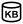
\includegraphics{KB-symbol-tiny.png}}}}

\makeatletter
\newcommand\mathcircled[1]{%
	\mathpalette\@mathcircled{#1}%
}
\newcommand\@mathcircled[3]{%
	\tikz[baseline=(math.base)] \node[draw,circle,inner sep=1pt] (math) {$\m@th#1#2$};%
}
\makeatother

\begin{document}
%
\title{Introducing Logic Transformer}
%
%\titlerunning{Abbreviated paper title}
% If the paper title is too long for the running head, you can set
% an abbreviated paper title here
%
% \author{$\blacksquare\blacksquare\blacksquare\blacksquare$}
\author{King-Yin Yan \orcidID{0009-0007-8238-2442}}
%
% \authorrunning{$\blacksquare\blacksquare\blacksquare\blacksquare$}
\authorrunning{K-Y. Yan}
% First names are abbreviated in the running head.
% If there are more than two authors, 'et al.' is used.
%
% \institute{$\blacksquare\blacksquare\blacksquare\blacksquare$}
\institute{\email{general.intelligence@gmail.com}}
%
\maketitle              % typeset the header of the contribution
%
\begin{abstract}
	Traditional Transformer-based models excel at pattern matching but struggle with compositional generalization and logical coherence, often leading to hallucinations in complex reasoning tasks. In this paper, we introduce the \textbf{Logic Transformer}, a novel differentiable neural architecture designed to explicitly perform classical symbolic logic inference (e.g., rule matching and variable substitution). Unlike traditional distributed representations, the Logic Transformer implements a continuous relaxation of symbolic operations. A key innovation is the \textit{cylindrification factor}, which allows logic constants to transition continuously into variables, enabling differentiable unification. Furthermore, we draw an algebraic parallel between our differentiable variable slots and the Self-Attention mechanism, providing a new categorical perspective on neural-symbolic integration. Preliminary experiments on logical reasoning tasks (e.g., bAbI) and language modeling (TinyStories) demonstrate that the Logic Transformer achieves competitive performance while requiring an order of magnitude fewer parameters than traditional Transformers. This high parameter efficiency, coupled with its explicit rule structure, offers a promising direction for building interpretable, resource-efficient, and logically coherent AI systems.
\end{abstract}

\keywords{Neurosymbolic AI \and Differentiable Logic \and Parameter Efficiency \and Compositional Generalization \and Logic Transformer}

%\begin{tikzpicture}[remember picture,overlay]
%\node[draw, rectangle, red] at ([shift={(8cm,-2cm)}]current page.north west) {\huge\textbf{NOTE: unfinished draft}};
%\end{tikzpicture}

\section{Introduction}
\label{sec:intro}
The success of Large Language Models (LLMs) based on the Transformer architecture \cite{Vaswani2017} has been unprecedented. However, their reliance on distributed, statistical representations inherently limits their ability to perform rigorous, multi-step logical reasoning. This often manifests as ``hallucinations'' and a failure in compositional generalization—the ability to combine known concepts into novel configurations \cite{Lake2018}.

To bridge the gap between the pattern-matching prowess of neural networks and the rigorous coherence of symbolic AI, we propose the \textbf{Logic Transformer}. Rather than treating logic as an emergent property of massive scale, we explicitly embed classical symbolic operations—such as rule matching and variable substitution—into the neural architecture via continuous relaxation.

The core contributions of this paper are:
\begin{itemize}
	\item We introduce a differentiable mechanism for logic rule matching, centered around a novel \textit{cylindrification factor} that smoothly transitions between constant matching and variable substitution.
	\item We formulate differentiable variable slots using Softmax-based attention, drawing a formal algebraic parallel to the Self-Attention mechanism via string diagrams.
	\item We demonstrate empirically that this explicit logical structure allows the Logic Transformer to achieve competitive performance on reasoning benchmarks (e.g., bAbI, TinyStories) with an order of magnitude fewer parameters than traditional Transformers.
\end{itemize}

\section{Logic Transformer}

In classical logic-based AI, a single step of inference is a mapping $ \Gamma \xmapsto{\kb} \Gamma + \delta $ where $\kb$ is a set of logic \textbf{rules} and $\Gamma$ is a set of ground propositions or \textbf{facts}.  $\Gamma$ also called the state $\vec{x}$ or Working Memory.  ``Set'' implies algebraic structure, ie, permutation invariance of elements.  We recognized early on that this has a connection with the \textbf{equivariant} structure of Self-Attention; but it was not obvious how to extract further algebraic structures from logic and to apply such symmetries; instead, we found a way to actually implement the syntactic operations of substitutions and logic-rule matching, so the resulting neural network obviously inherits logic structure implicitly.  A logic rule is a formula with variables such as: %\vspace{0.1cm}
\begin{equation}
	\forall X \; \forall Y \; \forall Z.  \quad \text{father}(\tikzmarknode{nX1}{{\color{gray}X}}, \tikzmarknode{nY1}{{\color{gray}Y}}) \wedge \mbox{father}(\tikzmarknode{nY2}{{\color{gray}Y}}, \tikzmarknode{nZ1}{{\color{gray}Z}})
	\Rightarrow \text{grandfather}(\tikzmarknode{nX2}{{\color{gray}X}}, \tikzmarknode{nZ2}{{\color{gray}Z}})
	\begin{tikzpicture}[remember picture,overlay,distance=1.1cm]
		\draw[-,thick,dotted,transform canvas={shift={(1pt,5pt)}}] (nX1.center) .. controls +(0cm,0.4cm) and +(-0cm,0.4cm) .. (nX2.center);
		\draw[-,thick,dotted,transform canvas={shift={(0pt,-5pt)}}] (nY1.center) .. controls +(0cm,-0.3cm) and +(0cm,-0.3cm) .. (nY2.center);
		\draw[-,thick,dotted,transform canvas={shift={(0pt,-5pt)}}] (nZ1.center) .. controls +(0cm,-0.3cm) and +(0cm,-0.3cm) .. (nZ2.center);
	\end{tikzpicture}
	\label{linkage-father}
\end{equation}
where the variables must obey strict discipline ($X$ matches to $X$, etc) as shown by dotted lines.

% ``Logic'' in quotes because, as I write this paper, I start to realize that neural associative memory (such as Transformer, which has been shown to be equivalent to Hopfield Networks \cite{Ramsauer2021}) may be a far superior form of ``logic'' than traditional, formal symbolic logic. % But I started this paper with differentiable symbolic logic, let's follow that idea.

% Finally I had a break-through insight that a symbolic-logic Transformer should output \textbf{atomic propositions} that modify a linguistic tree \textbf{at one position} at a time (Fig.\ref{fig:flat-vs-tree}).  Tree structure simplifies the implementation of logic rules -- fewer parameters needed; learns faster.  An analogy is that humans try to parse sentences syntactically first (which requires only superficial information such as parts-of-speech) before deeper semantic understanding.  In order words, grammar \textit{simplifies} subsequent understanding.

%\begin{figure}
%% NOTE: use ~/Downloads/GraphML-to-Tikz to convert graphML to Tikz, then edit Tikz
%\centering
%\begin{tikzpicture}[every path/.style={thick}]
%\begin{scope}[scale=2.5]
%\tikzstyle{defnode}=[draw,rectangle,rounded corners=4pt,node font=\small,inner ysep=1pt]
%
%\node (a) [defnode] at (-1, 0)   {I\strut};
%\node (b) [defnode] at (-0.5, 0) {love\strut};
%\node (c) [defnode] at (0, 0)    {you\strut};
%\node (d) [defnode] at (0.5, 0)  {to\strut};
%\node (e) [defnode] at (1, 0)    {pieces\strut};
%
%\foreach \n/\m in {a/b,a/c,a/d,a/e,b/c,b/d,b/e,c/d,c/e,d/e} {
%	\draw (\n.north) to[bend left] node[above] {} (\m.north); }
%\end{scope}
%\begin{scope}[shift={(5.5,0.2)},scale=1.5,rotate=-20]
%\tikzstyle{defnode}=[draw,rectangle,rounded corners=4,thick,node font=\small]
%\tikzstyle{defedge}=[->,thick]
%
%\node(I) at (-1,0)       [defnode] {I};
%\node(love) at (0,0)     [defnode] {love};
%\node(you) at (1,0)      [defnode] {you};
%\node(to) at (0,0.6)     [defnode,gray] {to};
%\node(pieces) at (1,0.6) [defnode,gray] {pieces};
%
%\draw[defedge](I) edge (love) (love) edge (you);
%\draw[defedge,gray] (to) edge (love) (to) edge (pieces);
%\end{scope}
%\end{tikzpicture}
%\caption{\textbf{Left:} In traditional Self-Attention Transformer, each token is related to every other token, ie. fully connected graph.  \textbf{Right:}  Example of a linguistic tree or graph, where only some nodes are connected.  From a \textbf{Chomskyan} perspective, any NL sentence can fit into a tree structure.  This example starts with a simple relation, I-love-you, and the ``love'' node is modified by a ``to'' clause (grey).  Let's not dwell too deep into this example, as machine-learning will fill in such details.}
%\label{fig:flat-vs-tree}
%\end{figure}

% Having convinced ourselves that LLMs can be a model of \textit{internal} thoughts, we wonder if the Transformer can be re-formulated as some kind of logic engine or general \textbf{rewriting system}, defined by rewriting \textbf{rules} that can be learned via gradient descent?

% \textbf{Knowledge Representation}. We may endow the KR structure with additional structures such as:  1) tree structure as inspired by Chomskyan linguistics; 2) ontology encoded as topological ordering (eg. ``cones'') in vector space; 3) probabilistic or fuzzy strength as the size of a thought vector.  This implies that thoughts are directions on a hypersphere, as some researchers have noted of Transformer tokens \cite{Pochinkov2023}.

% \textbf{Graph-rewriting}.  In \cite{Goertzel2021} \cite{Goertzel2021b}, Goertzel formulates intelligence as the re-writing of some metagraph or hypergraph structure, which is essentially the same as the author's idea of tree as Working Memory and which I now link to the Transformer.  Rewriting is defined categorically as certain morphisms, requiring some diagrams to commute.  This defines intelligence in \textbf{algebraic} terms, and it requires the discretizing functions above to achieve such algebraic rewriting.

% \textbf{The Rete algorithm} is another classical AI technique to accelerate rules-matching.  It is based on the observation that Working Memory changes incrementally, so one should find matchings from the ``delta'' change instead of the entire memory content.  In a sense we are re-tracing many classical AI ideas and adapting them to the new LLM setting.  In this case, we can learn a probabilistic function from Working Memory to rules which are most likely applicable.  This increases efficiency while still maintaining differentiability.

%{\color{red} Update:  need to handle \textbf{variable-length propositions}.  Need tree-rewriting logic.  In a certain direction, the neural network may end up with a form very close to or even identical to current Transformers.}
%\begin{equation}
%	\nonumber
%	\vcenter{\hbox{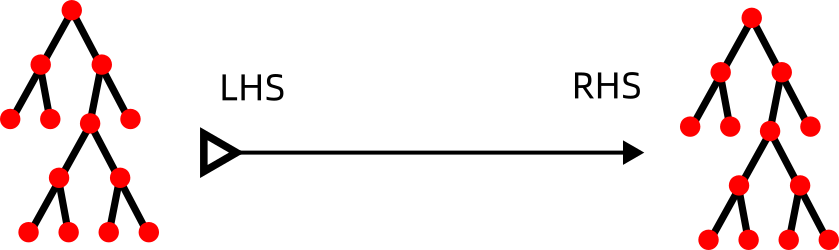
\includegraphics[scale=0.7]{tree-rewriting.png}}}
%\end{equation}

% Now we are ready to re-formulate the Transformer as applying a set of logic / symbolic rules to its inputs.  In order for such rules to be \textbf{differentiable}, we can't have $N$ rules at one moment and then suddenly $N+1$ rules the next moment (that would not be differentiable).  The only solution I can think of is to maintain a \textit{fixed} number, $M$, of rules.  Every rule may potentially ``morph'' into any other rule in this space of rules.  The set of rules would look like a \textit{rectangular} matrix: {\color{red}(This part needs modification for tree-based logic rules instead of fixed-length rules; Tree-based rules require special syntax.  This may not be too difficult, as tree-rewriting is equivalent to term-rewriting, which the author already has some familiarity with.  [Goertzel 2021] also developed a ``reflective metagraph rewriting as a foundation for an AGI language of thought'')}

%\begin{equation}
%\begin{aligned}
%\mbox{rule 1:} & \quad \boxed{X^1_{11}... X^1_{1I}} \;\wedge\; \boxed{X^1_{21} ... X^1_{2I}} \;\wedge\;...\; \boxed{X^1_{K1} ... X^1_{KI}} \rightarrow \boxed{X^1_{01} ... X^1_{0I}} \\
%\mbox{rule 2:} & \quad \boxed{X^2_{11}... X^2_{1I}} \;\wedge\; \boxed{X^2_{21} ... X^2_{2I}} \;\wedge\;...\; \boxed{X^2_{K1} ... X^2_{KI}} \rightarrow \boxed{X^2_{01} ... X^2_{0I}} \\
%.... & \quad .... \\
%\mbox{rule M:} & \quad \boxed{X^M_{11}... X^M_{1I}} \;\wedge\; \boxed{X^M_{21} ... X^M_{2I}} \;\wedge\;...\; \boxed{X^M_{K1} ... X^M_{KI}} \rightarrow \boxed{X^M_{01} ... X^M_{0I}}
%\end{aligned}
%\end{equation}

%For a rule to be applicable, its atoms must match with propositions in Working Memory.  An atom may contain constants (such as ``Socrates'', that must be matched correspondingly) or variables (such as $x$, that matches any entity).  To achieve this, I introduce a trick called \textbf{cylindrification factor} (Fig.\ref{fig:cylindrify-example}).

%\begin{figure}
%	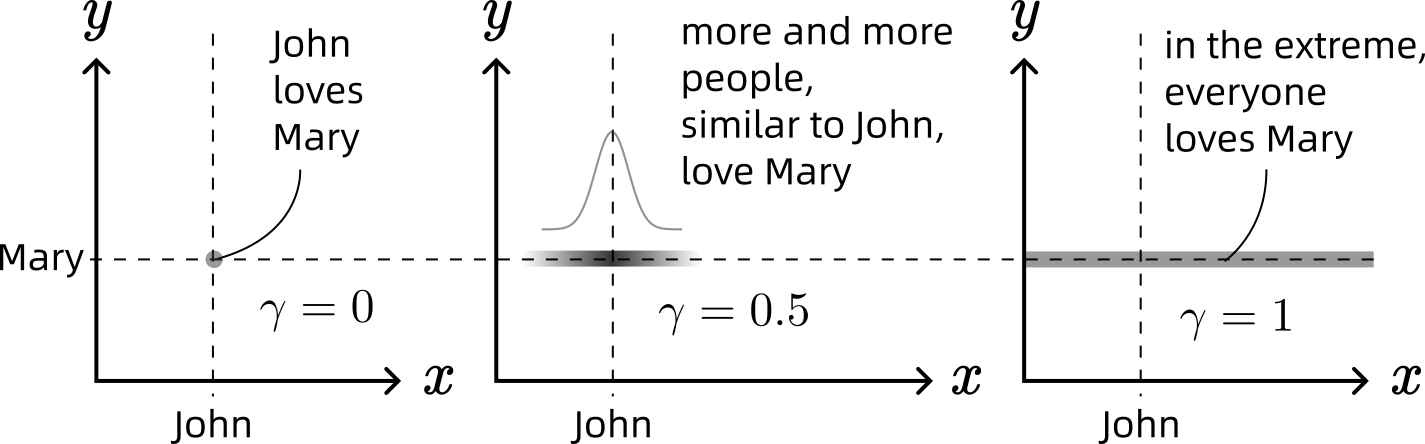
\includegraphics[scale=.6]{cylindrify-example.png}
%	\caption{Illustration of the cylindrification factor $\gamma$.}
%	\label{fig:cylindrify-example}
%\end{figure}

%\begin{equation}
%	\gamma =\begin{cases}
%		\approx 0 \Rightarrow \mbox{constant, do matching, TV = match degree} \cdot \sigmoid(1 - \gamma) \\
%		\approx 1 \Rightarrow \mbox{variable, do substitution, TV = 1} \cdot \sigmoid(\gamma)
%	\end{cases}
%\end{equation}
%Each position inside a rule can be either a constant or variable, and their treatments are obviously very different, but the results of the two streams would be super-imposed (added) together, pretty much like the \textbf{superposition} of quantum states.

%To make \textbf{variable substitution} differentiable is even trickier.  Consider this logic rule:
%\begin{equation}
%\logic{father}(X_1,X_2) \wedge \logic{father}(X_2,X_3) \rightarrow \logic{grand\hbox{-}father}(X_1,X_3)
%\end{equation}

%We have to imagine some ``slots'' where we ``select'' variables using weights and \textbf{softmax}:
%\vspace{-0.2cm} \begin{equation}
%\logic{father}(
\begin{tikzpicture} \draw[line width=3pt, gray!50] (0.2,0.9) -- (0.2,0) (0.5,0.9) -- (0.5,0) (0.8,0.2) -- (0.8,0); \draw[thick] (0,0) to (1,0); \end{tikzpicture})
%\wedge
%\logic{father}(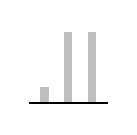
\begin{tikzpicture} \draw[line width=3pt, gray!50] (0.2,0.2) -- (0.2,0) (0.5,0.9) -- (0.5,0) (0.8,0.9) -- (0.8,0); \draw[thick] (0,0) to (1,0); \end{tikzpicture})
%\rightarrow
%\logic{grand\hbox{-}father}(
\begin{tikzpicture} \draw[line width=3pt, gray!50] (0.2,0.9) -- (0.2,0) (0.5,0.2) -- (0.5,0) (0.8,0.9) -- (0.8,0); \draw[thick] (0,0) to (1,0); \end{tikzpicture})
%\end{equation}

A key innovation is what I termed the \textbf{cylindrification factor} $\gamma$, which allows a logic constant to change continuously into a variable, as illustrated in fig. \ref{fig:cylindrification}.

\begin{figure}
%	\hspace{-3cm}
	\centering
	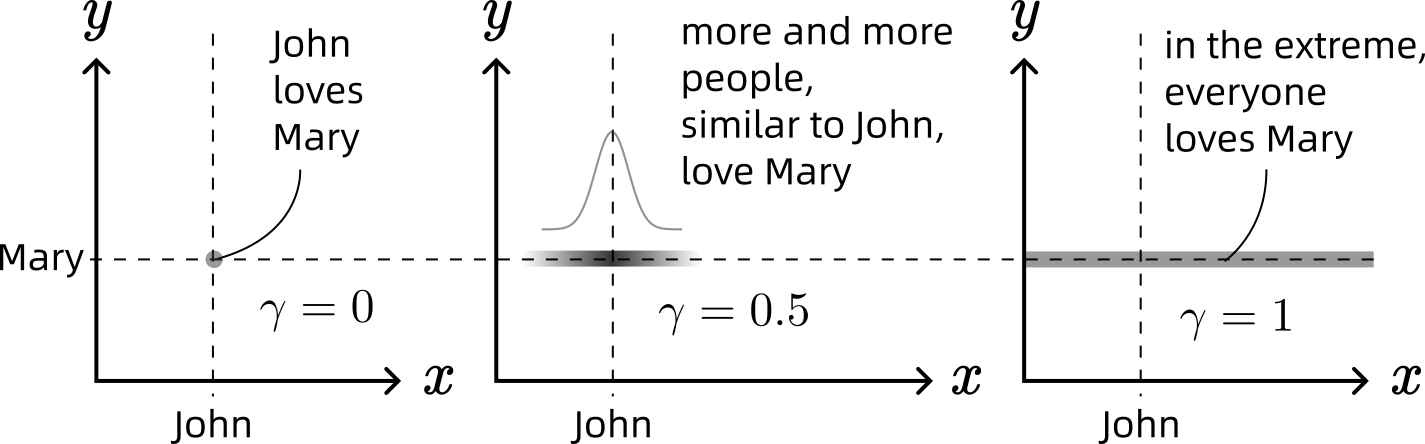
\includegraphics[scale=.5]{cylindrify-example.png}
	\caption{Illustration of the cylindrification factor $\gamma$.}
	\label{fig:cylindrification}
\end{figure}

%\textbf{Differentiable symbolic logic}.  In order to implement differentiable logic rules, I came up with a mechanism sort of like ``loading'' and ``unloading'' tokens into variable slots:
Furthering the idea, the matching (or \textbf{unification}) of variables makes use of a fixed number of variable ``slots'' where we ``move'' contents in and out of the slots by neural weights with \textbf{Softmax}, so that the transfer of contents can vary continuously:
\begin{align}
\nonumber
& \qquad \qquad \tikzmark{Y1}
\setlength{\fboxrule}{3pt}
\fcolorbox{gray!50}{white}{$\hat{x}^1$}
\qquad
\tikzmark{Y2} \fcolorbox{gray!50}{white}{$\hat{x}^2$}
\qquad
\tikzmark{Y3} \fcolorbox{gray!50}{white}{$\hat{x}^3$}
\hspace{3.4cm}
\tikzmark{Z1} \fcolorbox{gray!30}{white}{} \quad
\tikzmark{Z2} \fcolorbox{gray!30}{white}{} \quad
\tikzmark{Z3} \fcolorbox{gray!30}{white}{}
\\
\label{eqn:differentiable-variable-slots}
& \hspace{-0.2cm} \hat{W} = [ \hat{w}_{ij}^k ] \\
& \hspace{7.4cm} \check{W} = [ \check{w}^\ell_k ] \nonumber \\
& \logic{father}(\tikzmark{X11} x_{11}, \tikzmark{X12} x_{12}, \tikzmark{X13} {-}_{13}) \wedge
\logic{father}(\tikzmark{X21} {-}_{21}, \tikzmark{X22} x_{22}, \tikzmark{X23} x_{23}) \rightarrow \logic{grand\hbox{-}father}(\tikzmark{X1} x_1, \tikzmark{X2} {-}_2, \tikzmark{X3} x_3) .
\nonumber
\begin{tikzpicture}[remember picture,overlay]
\draw (pic cs:Y1) +(10pt,-7pt) -- ($ (pic cs:X11) +(7pt,10pt) $);
\draw (pic cs:Y1) +(10pt,-7pt) -- ($ (pic cs:X12) +(7pt,10pt) $);
\draw (pic cs:Y1) +(10pt,-7pt) -- ($ (pic cs:X13) +(7pt,10pt) $);
\draw (pic cs:Y1) +(10pt,-7pt) -- ($ (pic cs:X21) +(7pt,10pt) $);
\draw (pic cs:Y1) +(10pt,-7pt) -- ($ (pic cs:X22) +(7pt,10pt) $);
\draw (pic cs:Y1) +(10pt,-7pt) -- ($ (pic cs:X23) +(7pt,10pt) $);
\draw (pic cs:Y2) +(10pt,-7pt) -- ($ (pic cs:X11) +(7pt,10pt) $);
\draw (pic cs:Y2) +(10pt,-7pt) -- ($ (pic cs:X12) +(7pt,10pt) $);
\draw (pic cs:Y2) +(10pt,-7pt) -- ($ (pic cs:X13) +(7pt,10pt) $);
\draw (pic cs:Y2) +(10pt,-7pt) -- ($ (pic cs:X21) +(7pt,10pt) $);
\draw (pic cs:Y2) +(10pt,-7pt) -- ($ (pic cs:X22) +(7pt,10pt) $);
\draw (pic cs:Y2) +(10pt,-7pt) -- ($ (pic cs:X23) +(7pt,10pt) $);
\draw (pic cs:Y3) +(10pt,-7pt) -- ($ (pic cs:X11) +(7pt,10pt) $);
\draw (pic cs:Y3) +(10pt,-7pt) -- ($ (pic cs:X12) +(7pt,10pt) $);
\draw (pic cs:Y3) +(10pt,-7pt) -- ($ (pic cs:X13) +(7pt,10pt) $);
\draw (pic cs:Y3) +(10pt,-7pt) -- ($ (pic cs:X21) +(7pt,10pt) $);
\draw (pic cs:Y3) +(10pt,-7pt) -- ($ (pic cs:X22) +(7pt,10pt) $);
\draw (pic cs:Y3) +(10pt,-7pt) -- ($ (pic cs:X23) +(7pt,10pt) $);
\draw (pic cs:Z1) +(6pt,-7pt) -- ($ (pic cs:X1) +(7pt,10pt) $);
\draw (pic cs:Z1) +(6pt,-7pt) -- ($ (pic cs:X2) +(7pt,10pt) $);
\draw (pic cs:Z1) +(6pt,-7pt) -- ($ (pic cs:X3) +(7pt,10pt) $);
\draw (pic cs:Z2) +(6pt,-7pt) -- ($ (pic cs:X1) +(7pt,10pt) $);
\draw (pic cs:Z2) +(6pt,-7pt) -- ($ (pic cs:X2) +(7pt,10pt) $);
\draw (pic cs:Z2) +(6pt,-7pt) -- ($ (pic cs:X3) +(7pt,10pt) $);
\draw (pic cs:Z3) +(6pt,-7pt) -- ($ (pic cs:X1) +(7pt,10pt) $);
\draw (pic cs:Z3) +(6pt,-7pt) -- ($ (pic cs:X2) +(7pt,10pt) $);
\draw (pic cs:Z3) +(6pt,-7pt) -- ($ (pic cs:X3) +(7pt,10pt) $);
\draw[->,dotted] (pic cs:Y3) +(27pt,5pt) to [midway,sloped,"move to"] ($ (pic cs:Z1) +(-3pt,0pt) $);
\end{tikzpicture}
\end{align}
%\begin{equation}
%\hat{x}^k \mathrel{:}= \underset{\text{predicates}}{\forall i \in} \; \underset{\text{arguments}}{\forall j \in} \left\langle \mathrm{soft}\max_{ij} w_{ij}^k \; , \; x_{ij} \right\rangle
%\end{equation}
Interestingly, substitution / unification has a form very similar to \textbf{Self-Attention} except for the order of softmax and tensor product (with neural string-diagrams explained in the next section):
%\begin{equation}
%\text{Attention}(\mathbf{Q,K,V}) = \text{soft}\max  \frac{\langle \mathbf{Q,K} \rangle}{\sqrt{d_k}} \mathbf{V}
%\end{equation}
\begin{equation}
\begin{aligned}
\label{eqn:attention-string-diagrams}
	% \hat{x}^k \mathrel{:}= \underset{\substack{i \in \text{predicates} \\
	%	j \in \text{arguments}}}{\mathlarger{\forall}} \; \left\langle \mathrm{soft}\max_{ij} w_{ij}^k \; , \; x_{ij} \right\rangle
	Z \mathrel{:}= \sigmoid \check{W} \otimes \left( \sigmoid \hat{W} \otimes X \right)
	\qquad
	\def \globalscale {0.4}
	\vcenter{\hbox{\begin{tikzpicture}[y=1pt, x=1pt, yscale=\globalscale,xscale=\globalscale, every node/.append style={scale=\globalscale}, inner sep=0pt, outer sep=0pt]
	\begin{scope}[shift={(-115.59316, 283.87838)}]
		\path[draw=black,line width=0.8pt] (137.10858, -254.31339) -- (358.01601, -254.31339);

		\path[draw=black,line width=0.8pt] (137.32536, -153.20368) -- (244.69474, -153.20368).. controls (320.66437, -152.86162) and (318.7147, -271.01124) .. (245.63945, -271.5473) -- (186.27009, -271.5473);

		\path[draw=black,line width=0.8pt] (358.69474, -222.80075) -- (137.60239, -222.80075);

		\path[draw=black,line width=0.8pt] (137.93392, -204.9619) -- (222.34139, -204.9619).. controls (231.27231, -204.9619) and (238.46219, -197.77202) .. (238.46219, -188.8411) -- (238.46219, -187.64698).. controls (238.46219, -178.71606) and (231.27231, -171.52618) .. (222.34139, -171.52618) -- (138.21151, -171.52618);

		\path[draw=black,line width=0.8pt,->] (238.40059, -188.98504) -- (252.76995, -188.98504);

		\path[draw=black,line width=0.8pt,->] (301.05457, -209.88868) -- (315.42393, -209.88868);

		\path[draw=black,line width=0.8pt] (137.32536, -271.70366) -- (181.69471, -271.70366);

		\path[draw=black,fill=white,line width=0.8pt] (196.87486, -259.50278) -- (196.87486, -283.50282) -- (177.37495, -271.5028) -- cycle;

		\path[draw=black,fill=white,line width=0.8pt] (198.11309, -159.66386) -- (198.11309, -183.6639) -- (178.61318, -171.66388) -- cycle;

		\node[text=black,scale=2.8] at (123.30065, -158) {$\hat{W}$};
		\node[text=black,scale=2.8] at (122.17566, -213) {$X$};
		\node[text=black,scale=2.8] at (123.11316, -260) {$\check{W}$};

		\node[text=gray,scale=2] at (150, -145.84607) {$k$};
		\node[text=gray,scale=2] at (150, -163.22642) {$ij$};
		\node[text=gray,scale=2] at (150, -195.47644) {$ij$};
		\node[text=gray,scale=2] at (150, -215.16393) {$d$};
		\node[text=gray,scale=2] at (150, -245.16392) {$\ell$};
		\node[text=gray,scale=2] at (150, -264.66393) {$k$};

		\node[text=gray,scale=2] at (351.11322, -215.53932) {$d$};
		\node[text=gray,scale=2] at (351.11322, -247.03913) {$\ell$};

		\node[text=black,scale=1.6] at (190, -190.97644) {\textsf{Softmax}};
		\node[text=black,scale=1.6] at (190, -240.97644) {\textsf{Softmax}};

		\node[text=black,scale=1.6,align=center] at (270, -188) {\textsf{Mat}\\[-0.6em] \textsf{Mul}};
		\node[text=black,scale=1.6,align=center] at (331, -205) {\textsf{Mat}\\[-0.6em] \textsf{Mul}};
	\end{scope}
	\end{tikzpicture}}}
	\\
	\alpha \mathrel{:}= \left( \sigmoid \frac{\langle Q, K \rangle}{\sqrt{d_k}} \right) V
	\qquad
	\def \globalscale {0.4}
	\vcenter{\hbox{\begin{tikzpicture}[y=1pt, x=1pt, yscale=\globalscale,xscale=\globalscale, every node/.append style={scale=\globalscale}, inner sep=0pt, outer sep=0pt]
	\begin{scope}[shift={(-115.61316, 284.91126)}]
		\path[draw=black,line width=0.8pt] (137.10858, -267.14599) -- (323.51601, -267.14599).. controls (332.44696, -267.14599) and (339.63681, -261.45612) .. (339.63681, -252.5252) -- (339.63681, -251.33108).. controls (339.63681, -242.40016) and (332.44696, -235.21028) .. (323.51601, -235.21028) -- (279.88614, -235.21028);

		\path[draw=black,line width=0.8pt] (137.32536, -166.03628) -- (340.69473, -166.03628).. controls (419.47129, -165.99263) and (386.95878, -264.7707) .. (423.75002, -264.87989) -- (447.11938, -264.87989);

		\path[draw=black,line width=0.8pt] (137.32536, -235.63335) -- (166.4177, -235.63335).. controls (188.29528, -235.44173) and (178.67567, -217.85539) .. (200.93392, -217.7945) -- (222.34139, -217.7945).. controls (231.27231, -217.7945) and (238.46218, -210.60462) .. (238.46218, -201.6737) -- (238.46218, -200.47958).. controls (238.46218, -191.54866) and (231.27231, -184.35878) .. (222.34139, -184.35878) -- (138.21151, -184.35878)(265.69473, -235.63335) -- (200.60238, -235.63335).. controls (175.60248, -235.58176) and (191.56407, -217.84) .. (167.11898, -217.7945) -- (138.21151, -217.7945);

		\path[draw=black,line width=0.8pt,->] (238.40058, -201.81764) -- (306.76995, -201.81764);

		\path[draw=black,line width=0.8pt,->] (340.12491, -252.55318) -- (354.49427, -252.55318);

		\path[draw=black,line width=0.8pt] (137.32536, -284.53626) -- (447.19472, -284.53626);

		\path[draw=black,fill=white,line width=0.8pt] (285.37483, -223.58534) -- (285.37483, -247.58538) -- (265.87492, -235.58536) -- cycle;

		\node[text=black,scale=2.8] at (123.30065, -174.74652) {$Q$};
		\node[text=black,scale=2.8] at (122.17566, -225.37154) {$K$};
		\node[text=black,scale=2.8] at (123.11316, -276.93403) {$V$};

		\node[text=gray,scale=2] at (148, -158.67867) {$y$};
		\node[text=gray,scale=2] at (148, -176.05902) {$d$};
		\node[text=gray,scale=2] at (148, -208.30904) {$x$};
		\node[text=gray,scale=2] at (148, -227.99653) {$d$};
		\node[text=gray,scale=2] at (148, -257.99652) {$x$};
		\node[text=gray,scale=2] at (148, -277.49653) {$d$};

		\node[text=gray,scale=2] at (249.11315, -158.62153) {$y$};
		\node[text=gray,scale=2] at (249.11315, -228.37153) {$x$};

		\node[text=black,scale=1.6] at (206.11315, -202.30903) {\textsf{MatMul}};
		\node[text=black,scale=1.6] at (278.61316, -182.62154) {\textsf{Scale}  $* \sqrt{d}$};
		\node[text=black,scale=1.6] at (261.48817, -255.37153) {\textsf{Softmax}};

		\node[text=gray,scale=2] at (309.86317, -228.37153) {$x$};
		\node[text=gray,scale=2] at (309.86317, -260.62152) {$x$};

		\node[text=gray,scale=2] at (435, -256.87157) {$y$};
		\node[text=gray,scale=2] at (435, -274.87154) {$d$};

		\node[text=black,scale=1.6] at (369.73814, -234.74651) {\textsf{MatMul}};
	\end{scope}
\end{tikzpicture}}}
\end{aligned}
\end{equation}

The next step is to match Working Memory Elements (WMEs, i.e., propositions) to rule arguments. In classical symbolic AI, this matching process can lead to combinatorial explosion, a challenge historically addressed by algorithms like Rete \cite{Forgy1982}.

Instead of resorting to discrete, computationally prohibitive Cartesian self-products ($X^{\times n}$), the Logic Transformer employs a differentiable approximation. By leveraging the permutation invariance inherent in our architecture, we can efficiently compute the compatibility between WMEs and rule arguments through continuous tensor operations. This allows the network to learn a probabilistic mapping from Working Memory to the most applicable rules, maintaining differentiability while drastically reducing computational overhead.

An initial version of our system can solve TicTacToe quite efficiently.  Further testing confirmed that it can solve natural-language tasks such as bAbI \cite{Weston2015} and TinyStories \cite{Eldan2023} with 10x fewer parameters than traditional Transformers (Fig \ref{fig:experiments}L).  We attribute this efficiency to the logic structure inherent in the Logic Transformer neural network.

\begin{figure}
	\hspace{-0.5cm}
	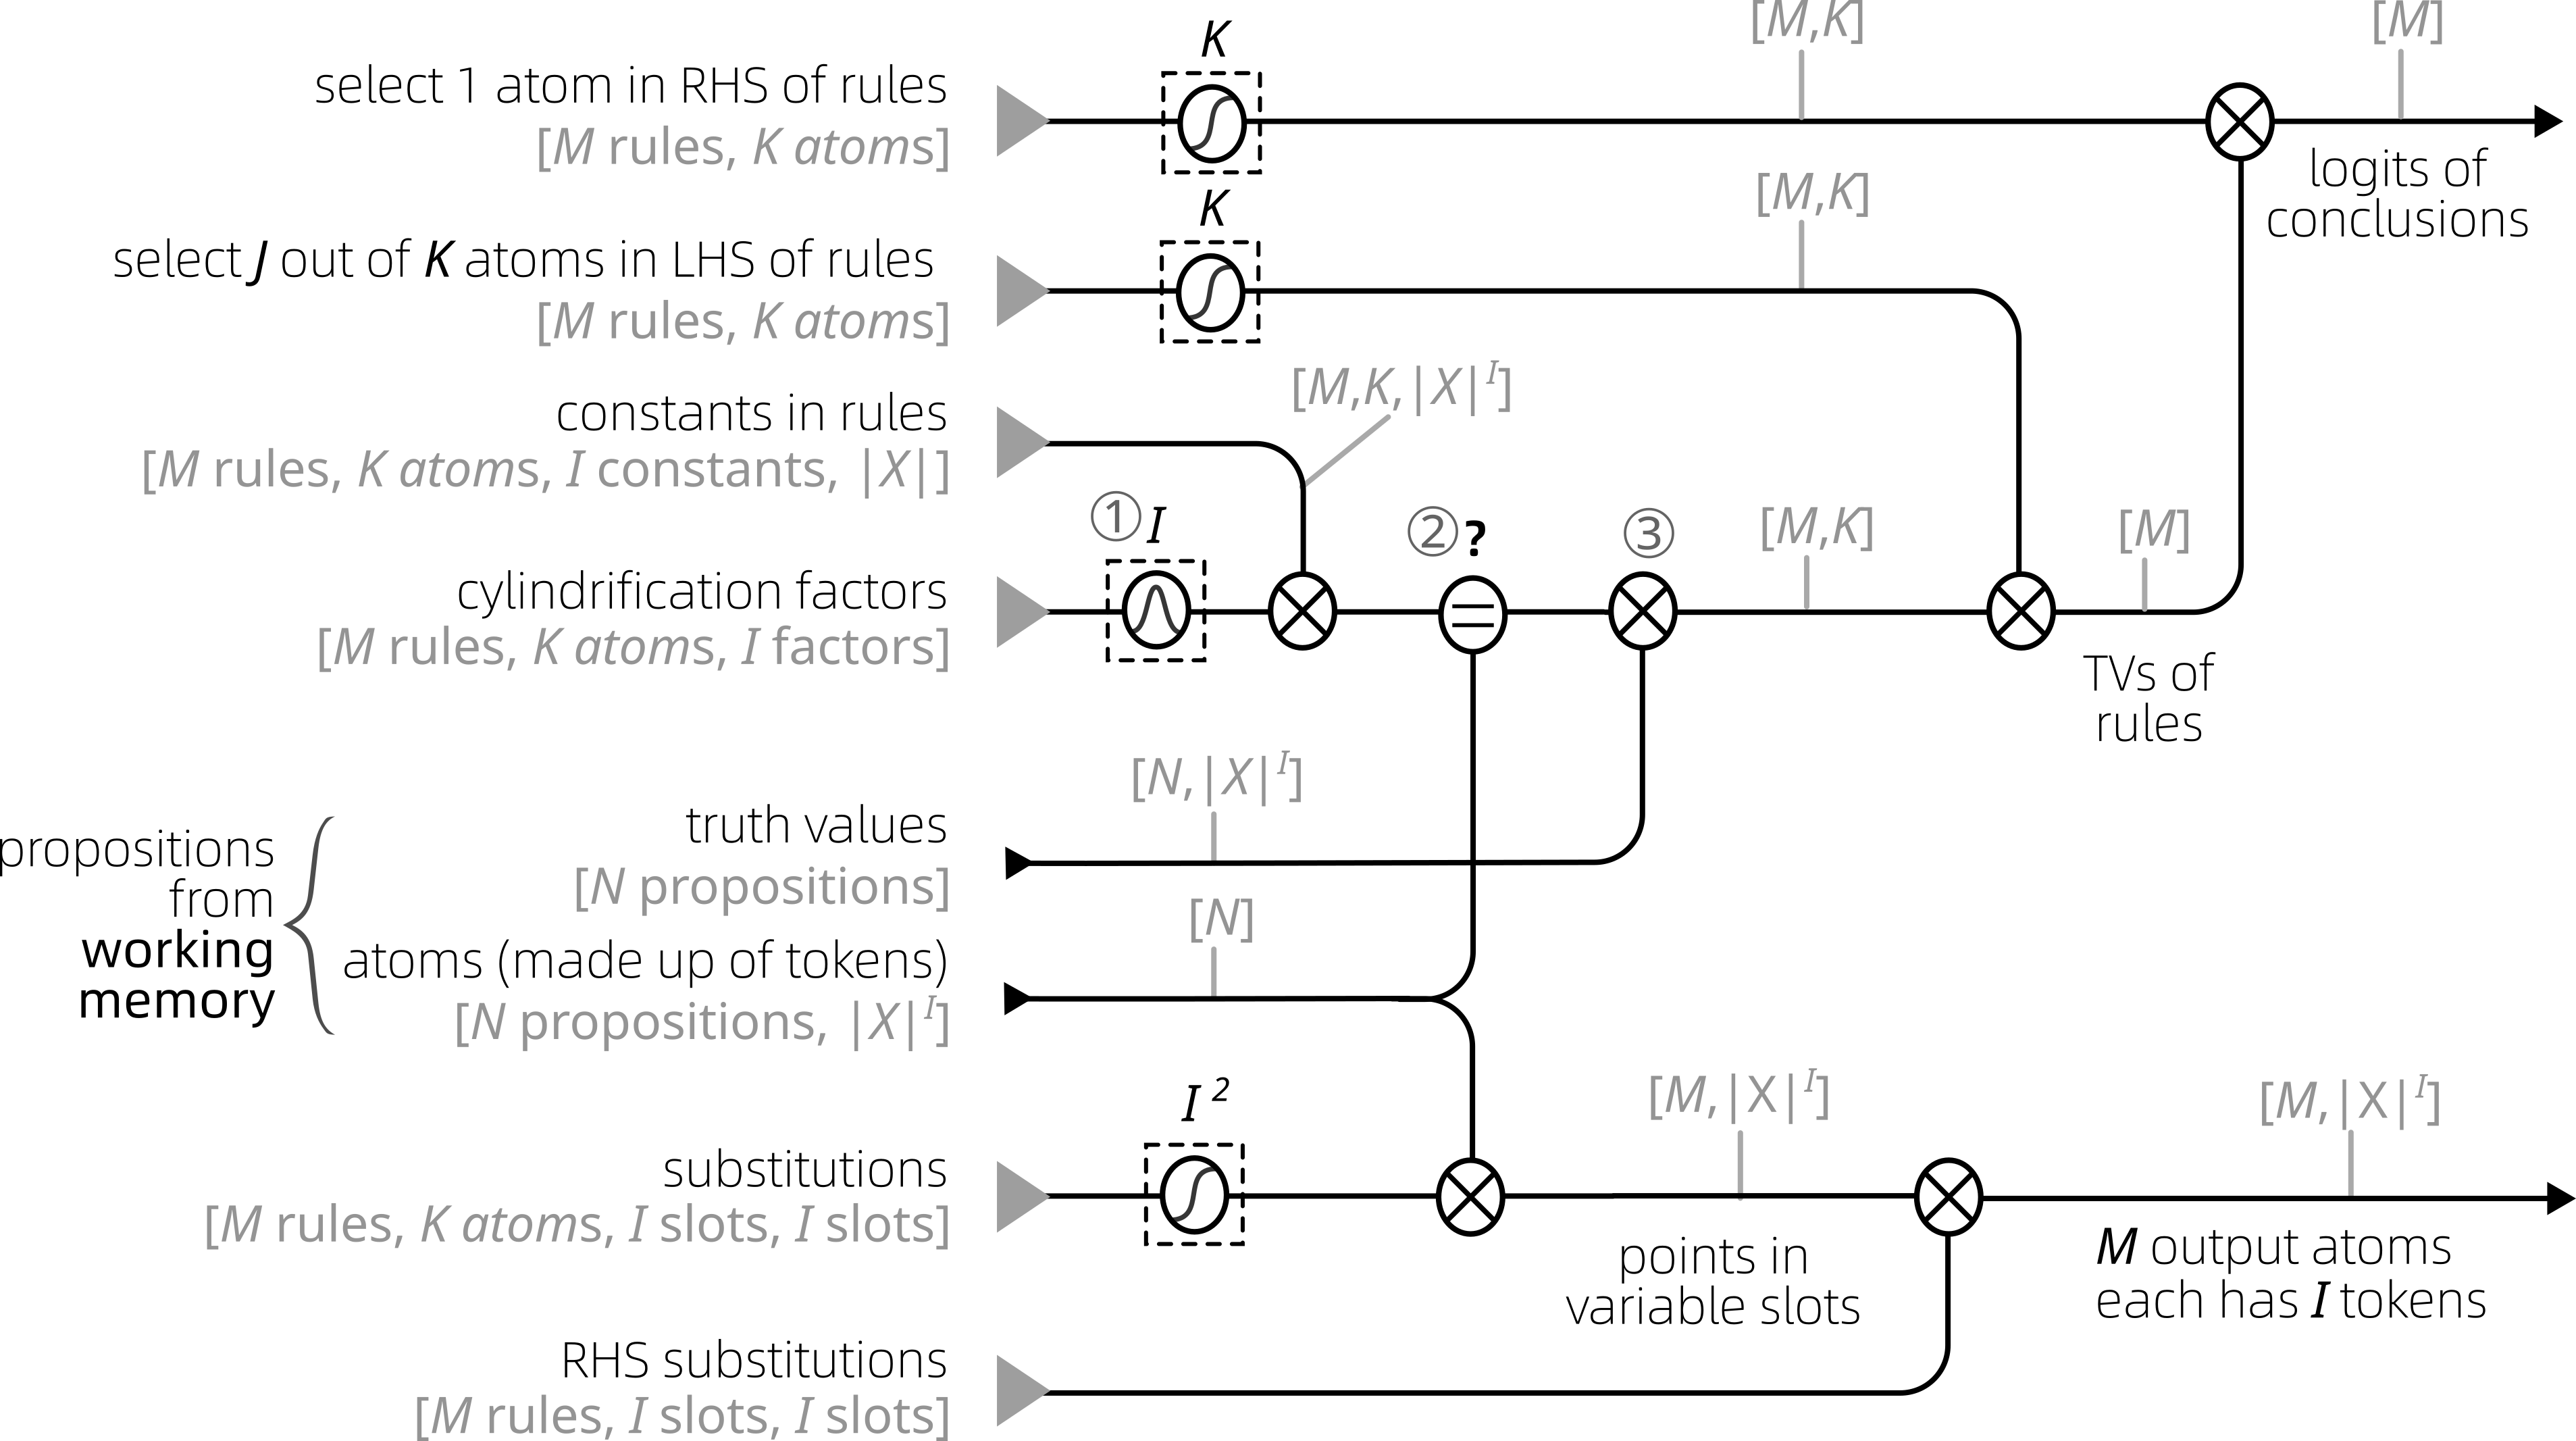
\includegraphics[scale=.5]{logic-Transformer-string-diagram-4b.png}
	\caption{String-diagram of the Logic Transformer.}
	\label{fig:logic-Transformer-string-diagram}
\end{figure}

\subsection{Source code and experiments}

We went through 3 stages of experiments. All source code is under Creative Commons Zero-1.0 license and can be accessed from: \\ \texttt{http://github.com/Cybernetic1/}\{insert name\}
\begin{center}
\begin{tabular}{|c|p{8cm}|p{4cm}|}
	\hline
	1 & TicTacToe experiments with traditional neural nets and Transformers & \texttt{RL-TTT-experiments} \\
	\hline
	2 & TicTacToe experiments with Logic Transformer & \texttt{logic-autoencoder-TTT} \\
	\hline
	3 & AGI experiments with bAbI and Tiny Stories & \texttt{AGI-experiments} \\
	\hline
\end{tabular}
\end{center}
Readers can use Copilot to ask questions about our code and even contribute new material. The repository is experimental code and contains >80 Markdown documents, mostly generated by Copilot, which may be difficult for beginners to navigate. Feel free to contact the author for assistance.

\begin{figure}
	\hspace{-0.2cm}
	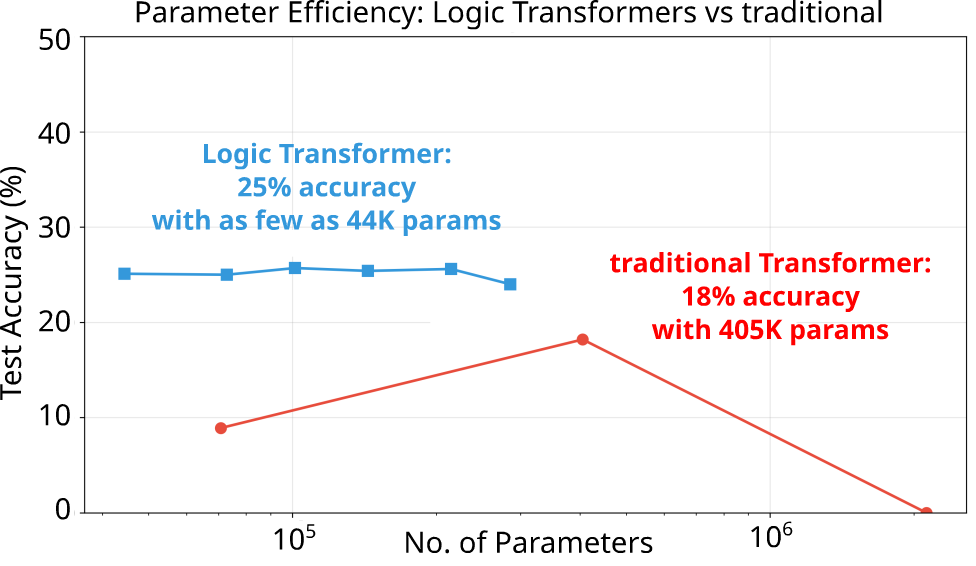
\includegraphics[scale=.25]{parameter_efficiency_comparison.png}
	\quad
	\raisebox{0.6cm}{
		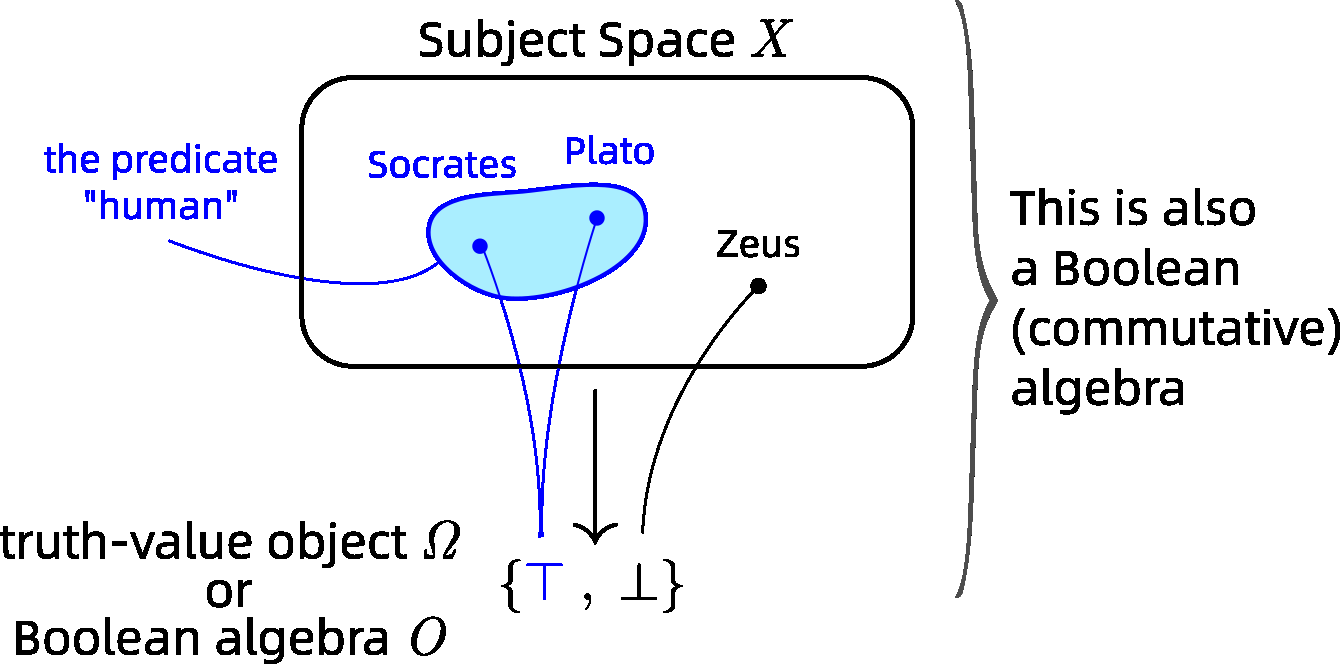
\includegraphics[scale=.32]{Halmos-nutshell.png}}
	\caption{(Left) Compression ratio, Logic Transformer vs traditional. (Right) Paul Halmos' lifting of propositional logic to predicate logic.}
	\label{fig:experiments} \label{fig:Halmos-nutshell}
\end{figure}

\subsection{On the algebraic structure of logic and string diagrams}

A natural question arises whether it is possible to simplify the string diagram (Fig. \ref{fig:logic-Transformer-string-diagram}) to make it computationally more efficient.  Some prior research has been done in this direction. The diagrams in equation (\ref{eqn:attention-string-diagrams}) are \textbf{Functor String Diagrams} as described in \cite{Abbott2024}. They have the advantage of keeping track of dimensions of tensors as well as preserving equivariant structure -- these seem to be all we need for implementing symbolic logic.

Let's digress a little into what we mean by ``logic structure.''  The modern approach is via categorical logic \cite{Jacobs1999} \cite{Lambek1986}, where logic structure is encapsulated as CCCs (\textbf{Cartesian closed categories}) or as \textbf{topoi} \cite{Goldblatt1984}.  The categorical approach has Curry-Howard correspondence \cite{Sorensen2006} at its core.  A parallel approach is based on relation algebra and leads to the notion of \textbf{allegories} \cite{Freyd1990}; it is inter-translatable with categorical logic.  Paul Halmos developed an early idea of algebraic logic based on lifting propositional logic to predicate logic via a morphism that preserves Boolean algebraic structure, as illustrated in Fig. \ref{fig:Halmos-nutshell}R. This idea is later developed into the notion of \textbf{hyperdoctrines} by Lawvere.

In the study of neural-symbolic integration, a central concern is the equivariant property $A \wedge B = B \wedge A$, which we believe is also a key feature of Self-Attention \cite{Vaswani2017} and thus Transformers.  The categorical way to capture permutation invariance is by \textbf{symmetric monoidal categories} (SMCs), which has the visual language of \textbf{string diagrams}.  \textbf{Compact closed} SMCs have dual objects and cup $\cup$ and cap $\cap$ morphisms. These allows to deal with operations such as tensor contraction (eg. dot product) -- required by the Attention mechanism.  We can \textbf{re-write} such string diagrams while preserving their symmetric / algebraic properties, eg \cite{Bonchi2022}. This sounds like a very exciting research direction, though unfortunately because the space of continuous functions has uncountable basis, the completeness of such rewriting cannot be guaranteed. What we have is equational completeness in the sense of $ \llbracket D_1 \rrbracket = \llbracket D_2 \rrbracket \Rightarrow D_1 \stackrel{*}{\leftrightarrow} D_2 $.

There is a path from SMCs $\rightarrow$ compact closed SMCs $\rightarrow$ Cartesian closed categories $\rightarrow$ topos, with increasingly more structure. We know how to construct neural networks in SMCs so the challenge is how to construct neural networks in toposes.  There is some research in this direction \cite{Spivak2014} \cite{Gavranovic2024}, which may shed light to our approach.

The string diagram in Fig. \ref{fig:logic-Transformer-string-diagram} is of an older style, as in \cite{Khatri2024}.  The model is impractical as it assumed the naive Cartesian product $X^n$ of Working Memory.  We are working with some modified version of it, but the claims of this paper remains basically truthful.

%but the rule (\ref{eqn:differentiable-variable-slots}) neglected the fact that the variables in each $\mathsf{father}$ atom must match their variables with each other (a situation well-known in classical logic-based AI).  This means we have to programmatically feed all \textit{pairs} of Working-Memory atoms, ie. the Cartesian product $A \times A$, into the above string diagram.  That makes it different from the Transformer which takes its input in plain form.  The reason why Transformer can do that is because it has many \textbf{layers}, and the matching of $A \times A$ can be achieved over these layers.

% except that softmax does not commute with inner products, so they are not exactly equivalent, but qualitatively similar.
% Indeed, neural \textbf{associative memory} (such as Transformer, which are shown to be equivalent to Hopfield Networks \cite{Ramsauer2021}) may be a far superior form of ``logic'' than traditional, formal symbolic logic.  Consider the logic example:
%\begin{equation}
%	\mbox{loves}(X, Y) \wedge \neg \mbox{loves}(Y,X) \rightarrow \frownie(X)
%\end{equation}
%but we immediately sense that the human brain does not work like that.  It is more like: the thought of unrequited love fires a massive number of neural activations which all point to the conclusion that this is an unhappy experience.  The Transformer's associative memory does exactly that.

% Let's pause for a moment to reflect that we tried to substitute variables (some kind of syntactic manipulation), and ended up with something like Self-Attention.
% Also recall that Self-Attention originated as a kind of \textbf{content-addressable memory} for Neural Turing Machines, invented for its differentiability.  In retrospect, it is also a very efficient implementation of associative memory.  If we want to improve the Transformer, we should first understand it as an associative memory.

% \textbf{Relation algebra}.  The matching of terms containing variables is combinatorially expensive - a fact well-known to an older generation of AI researchers.  To get around this problem, perhaps we can turn to relation algebra which has long established as a variable-free formalism.  For example, ``father's father is grandfather'' ($F; F = G$) is very close to human thinking.  I propose to extend beyond relations in the traditional sense, to a graphical knowledge representation where edges are ``linguistic'' relations.  For example: ``love and not loved back implies heartbreak'' ($\heartsuit ; \overline{\heartsuit}^\top \vdash \frownie$) does not mean that $\frownie$ is a relation with oneself; rather it is an inferred attribute, or unary predicate.  This example shows that the general rule about heartbreaks is independent of the individuals involved, as it should, and it has a form highly similar to relation algebra.  Inspired by Tarski's view that relation algebra can express most of mathematics\cite{Maddux2006} \cite{Schmidt2010}, we have grounds to believe that rewriting rules matching over linguistic graphs with labeled edges is plausibly powerful enough to express all of human intelligence.

% A final obstacle concerns the limitations of first-order logic.  As Ben Goertzel pointed out during an online discussion, my earlier design lacked mechanisms for handling \textbf{Skolem functions} and thus existential quantifiers.  One way to get around this problem is to define $\exists$ via a set of \textbf{higher-order logic} rules.  Without explicitly specifying how to do so (though I believe this can be done), we simply use a more powerful ``higher-order'' logic in the sense that rules admit substitutions in all (predicate or argument) positions, and hope that machine learning will learn the required axioms.

% Armed with these ideas, it is not too difficult to work out a new kind of differentiable ``Logic Transformer'' (Fig.\ref{fig:string-diagram}).  A detailed explanation is contained in my on-going research thesis \cite{YKY}.

%\begin{figure}
%	\hspace{-3cm}
%	\includegraphics[scale=.7]{logic-Transformer-string-diagram-3.png}
%	\caption{String diagram of the Logic Transformer.  The {\LARGE\color{gray}\RIGHTarrow} indicates \textbf{internal data} supplied by the Transformer, similar to the Q,K,V matrices in traditional Transformers.  These are modified through ``learning'' or training.  The 2 \RIGHTarrow's \ are \textbf{inputs} to the Transformer, this is matched with the 2 \textbf{outputs} on the right of the diagram.  Tags {\color{gray}$[M,N,...]$} indicate the \textbf{dimensions} of data streams.  {\color{red}NOTE:  diagram is obsolete as it pertains only to fixed-length propositions.}}
%	\label{fig:string-diagram}
%\end{figure}
%

% I guess I am not the only one among AGI researchers who is jealous of the success of the Self-Attention Transformer BERT-GPT lineage tradition.  Many like us suspect that Transformers are unnecessarily ``bulky'', meaning that they can be reduced or simplified.  But how?

% Functor $\mathsf{F}: \mathcal{C} \rightarrow \mathcal{D}$.
% From a \textbf{functorial} point of view (eg.\cite{Crescenzi2024} \cite{Abbott2024} \cite{Khatri2024}), one can find a functor that transforms a category $\mathcal{C}$ of KR structure and rewrite morphisms into another category $\mathcal{D}$ with different KR structure and rewrite morphisms.  It might just happen that one type of rewrite morphisms are computationally less costly than the other type, and so we have discovered a better, more efficient AGI system.  But this maneuver seems not so useful in light of the fact that Transformer / Self Attention is a distributive associative memory that may not care too much about its input representation.

% String diagrams allow us to visually compare architectures, such as Self-Attention with my differentiable Logic Transformer.  These diagrams can be ``morphed'' by rewriting rules.  One research team proposed universal approximators as an equivalence class of architectures under rewriting, but such a class is too permissive and pretty useless.  We want a more refined view of architectures such that we can distinguish which ones are more \textbf{learning-efficient} -- the key question in AGI development.

% If all continuous functions are equivalent, then what sets them apart?  My idea is that functions such as sigmoid and softmax are ``tearing'' the input space irreversibly, due to finite precision, into \textbf{discrete} regions that are no longer connected.  This process is crucial to eg. Transformer's ability to output discrete tokens.

% In Ben Goertzel's ``General Theory of General Intelligence'', he formulates intelligence as the re-writing of some metagraph or hypergraph structure, which is essentially the same as my idea of tree as Working Memory and which I now link to the Transformer.  Rewriting is defined categorically as certain morphisms, requiring some diagrams to commute.  This defines intelligence in \textbf{algebraic} terms, and it requires the discretizing functions above to achieve such algebraic rewriting.

% But the Transformer has also been shown capable of discrete (syntactic) manipulations.  Does that mean that all functions with discretizing ability are equivalent?  Can the Transformer be replaced by a fully-connected NN with sigmoid activation?  Seems unlikely, and if not, then what sets them apart \textit{still}?  Well, an obvious answer is that we need to \textbf{count computations}.

\section{Discussion and Future Directions}
\label{sec:discussion}
The explicit logical structure of the Logic Transformer opens several promising avenues for future research:

\textbf{Hybrid Neurosymbolic Architectures:} Because the learned logic rules in our model are cleanly separable entities, the neural network can seamlessly cooperate with traditional symbolic inference engines (e.g., Prolog or OpenCog). This allows for the rapid, zero-shot incorporation of new symbolic knowledge (e.g., algebraic axioms) directly into the reasoning process, bypassing the need for opaque, long-range dependency learning in traditional LLMs.

\textbf{Interpretability and Reflection:} Unlike the black-box nature of standard Transformers, the activation of specific rule parameters in the Logic Transformer can be directly inspected. This facilitates ``reflection,'' where inference traces can be made into inspectable objects, allowing the system (or human auditors) to verify the logical coherence of its thought processes.

\textbf{Algebraic Logic and String Diagrams:} As discussed in Section \ref{sec:algebra}, the functorial nature of our architecture suggests a deep connection to Symmetric Monoidal Categories (SMCs). Future work will explore optimizing the string diagram representations to further enhance computational efficiency while preserving equivariant structures.

\appendix

\section{Categorical Foundations and String Diagrams: A Beginner's Guide}
\label{app:category}

For readers unfamiliar with category theory, this appendix provides an intuitive introduction to Symmetric Monoidal Categories (SMCs), string diagrams, and the profound categorical insights that underpin the Logic Transformer.

\subsection{Intuition: Why Category Theory for Neural Networks?}
Modern deep learning frameworks fundamentally operate on directed acyclic graphs of tensor operations. Category theory provides the rigorous mathematical foundation for such graphs.
In the context of neural networks:
\begin{itemize}
	\item \textbf{Objects} represent \textit{tensor spaces} (e.g., vector spaces $\mathbb{R}^n$).
	\item \textbf{Morphisms} represent \textit{computations or layers} mapping one tensor space to another.
	\item \textbf{Composition} ($\circ$) represents \textit{sequential execution}.
	\item \textbf{Tensor Product} ($\otimes$) represents \textit{parallel execution}.
\end{itemize}

\subsection{Logical Conjunction: Cartesian vs. Tensor Products}
In classical logic, the conjunction ($\wedge$) is naturally modeled by the categorical product (Cartesian product) in a Cartesian Closed Category (CCC). However, in the context of neural networks, representations are often combined via the tensor product ($\otimes$).
A key insight of our work is that in certain Topoi or Symmetric Monoidal Categories, the strict Cartesian product can be continuously relaxed into a tensor product. This categorical flexibility is precisely what allows the Logic Transformer to bridge the gap between rigid symbolic logic (where $A \wedge B$ is discrete and strict) and distributed neural representations (where features are entangled via $\otimes$). The \textit{cylindrification factor} $\gamma$ introduced in the main text can be viewed as the algebraic parameter that navigates this relaxation.

\subsection{Categorical Databases, Sheaves, and Logical Instances}
A profound connection emerges when we view logical knowledge bases through the lens of categorical databases \cite{Spivak2014}.
\begin{itemize}
	\item A logical schema (e.g., the ontology of predicates and variables) can be formalized as a category $\mathcal{C}$.
	\item A specific state of the Working Memory (a set of grounded logical propositions) is then a \textbf{set-valued functor} $F: \mathcal{C} \to \mathbf{Set}$, which maps the abstract schema to concrete data instances, much like a database instance populates a database schema.
\end{itemize}
When we impose logical consistency constraints (e.g., via our differentiable rule matching and sandbox verification), we are effectively defining a Grothendieck topology on $\mathcal{C}$. The valid, logically coherent states of the neural network naturally form a \textbf{Sheaf} over this site. This sheaf structure guarantees that local logical consistencies can be uniquely ``glued'' together into a globally coherent thought process. We believe this topological perspective provides the ultimate mathematical antidote to hallucinations.

\subsection{Functor String Diagrams and Tensor Contraction}
To visually track the symmetries of variables and the flow of dimensions, we adopt the \textbf{Functor String Diagrams} recently formalized by \cite{Abbott2024}. Unlike traditional string diagrams where wires merely represent abstract objects, functor string diagrams explicitly label wires with their tensor dimensions, allowing us to trace the exact algebraic type of every data stream.

A particularly elegant feature of this formalism is the visualization of \textbf{tensor contraction}. In these diagrams, contracting two tensors of matching dimensions is represented by ``bending'' the wires to connect them, effectively ``annihilating'' the intermediate dimensions via cup ($\cup$) and cap ($\cap$) morphisms in a compact closed SMC.
\begin{itemize}
	\item Notably, the \textbf{dot product} is simply a special case of tensor contraction.
	\item The permutation invariance (equivariance) of our Logic Transformer's variable slots is perfectly captured by these diagrams: because the string diagrams are topologically invariant under the continuous deformation of wires (isotopy), the algebraic equivalence of logical permutations is guaranteed visually.
	\item Crucially, this rigorous dimensional tracking provides a perfect graphical representation of equivariance \textit{without} the need for ad-hoc coloring or manual tracking of variables.
\end{itemize}

\begin{figure}[h]
	\centering
	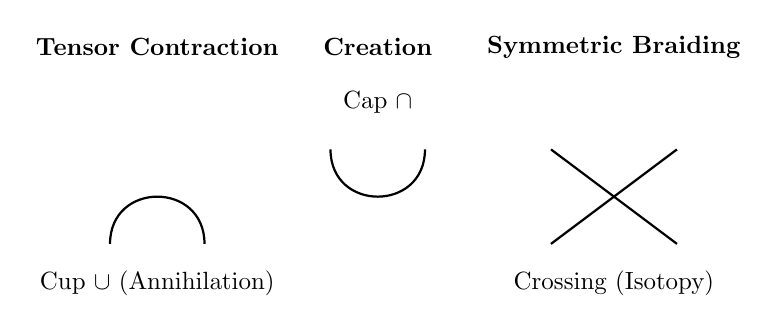
\begin{tikzpicture}[
		every node/.append style={scale=0.9},
		wire/.style={thick}
		]
		% --- Cup (Contraction) ---
		\node at (0, 2.5) {\textbf{Tensor Contraction}};
		\draw[wire] (-0.6,0) .. controls (-0.6, 0.8) and (0.6, 0.8) .. (0.6,0);
		\node at (0, -0.5) {Cup $\cup$ (Annihilation)};

		% --- Cap (Creation) ---
		\node at (2.8, 2.5) {\textbf{Creation}};
		\draw[wire] (2.2,1.2) .. controls (2.2, 0.4) and (3.4, 0.4) .. (3.4,1.2);
		\node at (2.8, 1.8) {Cap $\cap$};

		% --- Braiding (Permutation / Equivariance) ---
		% 【修正部分】：用标准的两条线交叉（Braiding）代替错误的 cross out 节点
		\node at (5.8, 2.5) {\textbf{Symmetric Braiding}};
		\draw[wire] (5.0, 0) to (6.6, 1.2);
		\draw[wire] (5.0, 1.2) to (6.6, 0);
		\node at (5.8, -0.5) {Crossing (Isotopy)};
	\end{tikzpicture}
	\caption{Topological representation of tensor operations in SMCs. Left \& Middle: Tensor contraction (e.g., dot product) via cup and cap morphisms. Right: Symmetric braiding (permutation of variables). The topological invariance of these diagrams under continuous deformation (isotopy) visually guarantees the permutation invariance of logical variables.}
	\label{fig:cup-cap-contraction}
\end{figure}

By framing the Logic Transformer in this categorical language, we ensure that the differentiable relaxation of symbolic logic strictly preserves the underlying algebraic symmetries of the knowledge base, paving the way for truly interpretable and mathematically grounded AGI architectures.

\subsection{The Visual Language of String Diagrams}
String diagrams are a topological visual language for SMCs. They allow us to "see" the algebraic structure of neural architectures without getting bogged down in index notation. The syntax is remarkably simple:
\begin{itemize}
	\item \textbf{Wires} represent data flows (tensors). The thickness or label of a wire indicates the dimension of the tensor.
	\item \textbf{Nodes (or Boxes)} represent operations (morphisms).
	\item \textbf{Plugging wires together} represents sequential composition.
	\item \textbf{Placing diagrams side-by-side} represents the tensor product (parallel computation).
	\item \textbf{Crossing wires} represents the \textit{symmetric braiding}, i.e., permuting the order of tensor dimensions.
\end{itemize}

\begin{figure}[h]
	\centering
	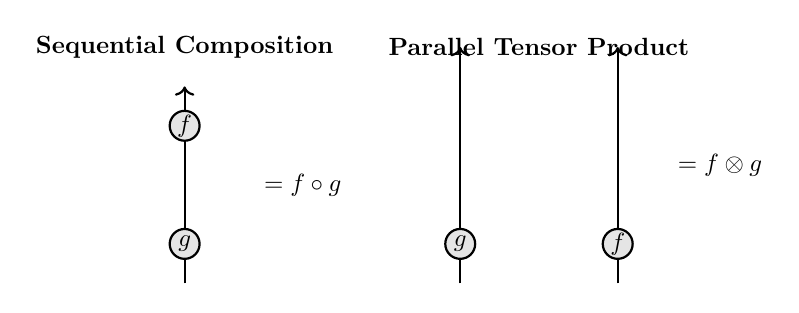
\begin{tikzpicture}[
		every node/.append style={scale=0.9},
		wire/.style={thick},
		op/.style={draw, circle, fill=gray!20, minimum size=12pt, inner sep=0pt}
		]
		% --- Composition (f \circ g) ---
		\node at (0, 2.5) {\textbf{Sequential Composition}};
		\draw[wire] (0,0) node[op] (g) {$g$} -- (0,1.5) node[op] (f) {$f$};
		\draw[wire] (0,-0.5) -- (g);
		\draw[wire, ->] (f) -- (0, 2.0);
		\node at (1.5, 0.75) {$= f \circ g$};

		% --- Tensor Product (f \otimes g) ---
		\node at (4.5, 2.5) {\textbf{Parallel Tensor Product}};
		\draw[wire] (3.5,0) node[op] (g1) {$g$} -- (3.5, 2.0);
		\draw[wire] (5.5,0) node[op] (f1) {$f$} -- (5.5, 2.0);
		\draw[wire] (3.5,-0.5) -- (g1);
		\draw[wire] (5.5,-0.5) -- (f1);
		\draw[wire, ->] (g1) -- (3.5, 2.5);
		\draw[wire, ->] (f1) -- (5.5, 2.5);
		\node at (6.8, 1.0) {$= f \otimes g$};
	\end{tikzpicture}
	\caption{Basic syntax of string diagrams. Left: Sequential composition. Right: Parallel tensor product.}
	\label{fig:string-diagram-basics}
\end{figure}

\subsection{Permutation Invariance and Equivariance}
A defining feature of the Logic Transformer (and traditional Self-Attention) is \textbf{permutation invariance} with respect to the Working Memory (e.g., the logical conjunction $A \wedge B$ is equivalent to $B \wedge A$).

In the language of SMCs, permutation invariance means that the string diagram representing the computation must be \textit{topologically invariant} under the crossing of wires (symmetric braiding). Traditional Transformers achieve this implicitly through the dot-product and softmax. In the Logic Transformer, we explicitly construct morphisms that respect this equivariant structure.

\subsection{Compact Closed SMCs and Tensor Contraction}
To implement operations like the dot product (which is central to both Self-Attention and our differentiable variable slots), we require a richer structure called a \textbf{Compact Closed SMC}.
In a compact closed category, every object $A$ has a dual object $A^*$. This allows for the existence of "cup" ($\cup$) and "cap" ($\cap$) morphisms, which visually represent \textbf{tensor contraction} (e.g., summing over a shared index).

\begin{figure}[h]
	\centering
	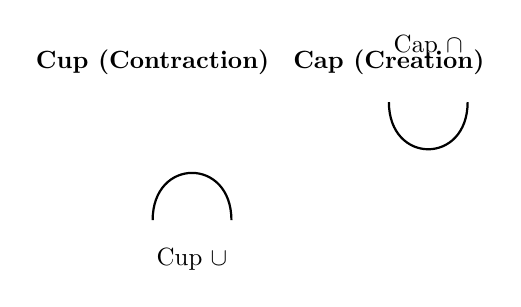
\begin{tikzpicture}[
		every node/.append style={scale=0.9},
		wire/.style={thick}
		]
		% --- Cup and Cap ---
		\node at (0, 2) {\textbf{Cup (Contraction)}};
		\draw[wire] (0,0) .. controls (0, 0.8) and (1, 0.8) .. (1,0);
		\node at (0.5, -0.5) {Cup $\cup$};

		\node at (3, 2) {\textbf{Cap (Creation)}};
		\draw[wire] (3,1.5) .. controls (3, 0.7) and (4, 0.7) .. (4,1.5);
		\node at (3.5, 2.2) {Cap $\cap$};
	\end{tikzpicture}
	\caption{Topological representation of tensor contraction (dot product) in compact closed SMCs.}
	\label{fig:cup-cap}
\end{figure}

The \textit{cylindrification factor} $\gamma$ and the Softmax-based variable loading mechanism introduced in Section 2 can be rigorously formalized as specific parameterized morphisms within this compact closed SMC. By framing our architecture in this way, we ensure that the differentiable relaxation of symbolic logic strictly preserves the underlying algebraic symmetries of the knowledge base.

\printbibliography

\end{document}
